\documentclass[12pt, twoside]{article}
\usepackage[letterpaper, margin=1in, headsep=0.5in]{geometry}
\usepackage[english]{babel}
\usepackage[utf8]{inputenc}
\usepackage{amsmath}
\usepackage{amsfonts}
\usepackage{amssymb}
\usepackage{tikz}
\usetikzlibrary{quotes, angles}
\usepackage{graphicx}
\usepackage{enumitem}
\usepackage{multicol}
\usepackage{hyperref}

\newif\ifmeta
\metatrue %print standards and topics tags

\title{IB Mathematics}
\author{Chris Huson}
\date{September 2021}

\usepackage{fancyhdr}
\pagestyle{fancy}
\fancyhf{}
\renewcommand{\headrulewidth}{0pt} % disable the underline of the header
\raggedbottom


\fancyhead[LE]{\thepage}
\fancyhead[RO]{\thepage \\ Name: \hspace{4cm} \,\\}
\fancyhead[LO]{BECA / IB Math 02-Descriptive Stats\\* 1 December 2021}

\begin{document}

\subsubsection*{2.4 Review: I can model arithmetic sequences}
Simple interest: $I=Crt$
\begin{enumerate}

\item The rate on a credit card is $18\%$ per annum. Find the interest due on a \$400 purchase after one month. \vspace{3cm}

\item Expand the following expression:\\
  $\displaystyle \sum_{n=1}^3 (3n+1)=$ \vspace{2cm}

Equations of a straight line: $f(x)=mx+c$, $ax+by+d=0$, $(y-y_1)=m(x-x_1)$\\[0.25cm]
Gradient: $\displaystyle m=\frac{y_2-y_1}{x_2-x_1}$ \vspace{0.5cm}
  
\item Given the linear function $f(x)=-x+5$.
\begin{multicols}{2}
\begin{enumerate}
  \item Write down it's slope.\\ $m=$
  \vspace{0.25cm}
  \item Write down it's $y$-intercept.\\ $b=$
  \vspace{0.25cm}
  \item Draw the function $f$ on the grid.
  \vspace{1cm}
  \item Label the $x$-intercept with its coordinates as an ordered pair.
\end{enumerate} \vspace{.5cm}
  \begin{center} 
  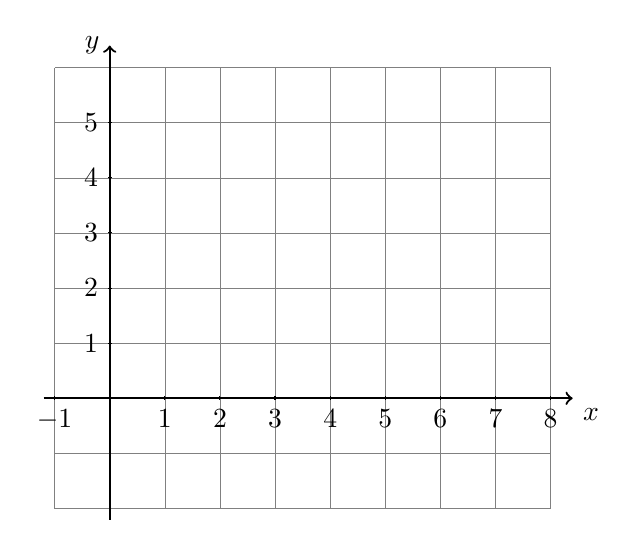
\begin{tikzpicture}[scale=0.7]
    \draw [help lines] (-1,-2) grid (8,6);
    \draw [thick, ->] (-1.2,0) -- (8.4,0) node [below right] {$x$};
    \draw [thick, ->] (0,-2.2)--(0,6.4) node [left] {$y$};
    \foreach \x in {-1,1,2,...,8} \draw (\x cm,1pt) -- (\x cm,-1pt) node[anchor=north] {$\x$};
    \foreach \y in {1, 2, 3, 4, 5} \draw (1pt,\y cm) -- (-1pt,\y cm) node[anchor=east] {$\y$};
    %\draw [thick, <->,smooth,samples=20,domain=-2.25:4.5] plot(\x,0.667*\x+2);
    %\fill (3,4) circle[radius=0.1] node[below right]{$Q$};
  \end{tikzpicture}
  \end{center}
\end{multicols}

\item Find the slope of the line through the points $A(-1,3)$, $B(4,-7)$.

\newpage
Arithmetic sequences\\[0.25cm]
Terms: $u_n=u_1 + d(n-1)$\\[0.25cm]
Sum: $\displaystyle S_n= \frac{n}{2}(u_1 + u_n)$\\[0.25cm]


\item Given the arithmetic sequence $12,8,4,0,-4, \dots$
  \begin{enumerate}[itemsep=1cm]
    \item Find the common difference $d$.
    \item Write down the next term, $u_6$.
    \item Find the nineth term.\vspace{1cm}
    \item Find the sum of the first nine terms.
  \end{enumerate} \vspace{2cm}

\item In an arithmetic sequence the first term is 6 and the fourth term is 24.
  \begin{enumerate}[itemsep=2cm]
    \item Find the common difference $d$.
    \item Find the tenth term, $u_{10}$.\vspace{1cm}
    \item Find the sum of the first ten terms.
  \end{enumerate} \vspace{3cm}


\end{enumerate}
\end{document}